\documentclass[12pt]{scrartcl}
\usepackage[german, ngerman]{babel}
\usepackage{graphicx}
\usepackage{color}
\usepackage{url}
\usepackage{xcolor}
\usepackage{listings}
\usepackage{hyperref}
\usepackage{nameref}
\usepackage{varioref}
\hypersetup{
    colorlinks=true,
    linkcolor={black!50!black},
    % linkcolor={red!50!black},
    citecolor={black!50!black},
    urlcolor={black!50!black}
}
\usepackage[headsepline,footsepline]{scrlayer-scrpage}
\usepackage{biblatex}
\usepackage{amsmath}
\usepackage{float}

\newcommand{\code}[1]{\texttt{#1}}


\definecolor{mGreen}{rgb}{0,0.6,0}
\definecolor{mGray}{rgb}{0.5,0.5,0.5}
\definecolor{mPurple}{rgb}{0.58,0,0.82}
\definecolor{backgroundColour}{rgb}{0.95,0.95,0.95} %{cmyk}{0.05,0.05,0.05,0.05}

\lstdefinestyle{CStyle}{
    backgroundcolor=\color{backgroundColour},
    commentstyle=\color{mGreen},
    keywordstyle=\color{blue},
    numberstyle=\tiny\color{mGray},
    stringstyle=\color{mPurple},
    basicstyle=\footnotesize,
    breakatwhitespace=false,
    breaklines=true,
    captionpos=b,
    keepspaces=true,
    numbers=left,
    numbersep=5pt,
    showspaces=false,
    showstringspaces=false,
    showtabs=false,
    tabsize=2,
    language=C++
}

\lstdefinestyle{Terminal}{
    backgroundcolor=\color{backgroundColour},
    commentstyle=\color{black},
    keywordstyle=\color{black},
    numberstyle=\tiny\color{black},
    stringstyle=\color{black},
    basicstyle=\footnotesize,
    breakatwhitespace=false,
    breaklines=true,
    captionpos=b,
    keepspaces=true,
    numbers=none,
    numbersep=5pt,
    showspaces=false,
    showstringspaces=false,
    showtabs=false,
    tabsize=2,
}


\pagestyle{scrheadings}
\clearscrheadfoot
%\cfoot{Tobias Gruber}
\cfoot{\pagemark}
\chead{\headmark}
\automark[subsection]{section}


\begin{document}


\begin{titlepage}
    \vfill
	\centering
    \vspace{1.5cm}

	{\scshape\LARGE Hochschule München \par}
    {\scshape\Large Fakultät für Informatik und Mathematik\par}
	\vspace{1.5cm}




    \vfill
    {\LARGE\bfseries Praktikumsaufgabe 3 \\}
    \vspace{0.5cm}
	{in der Vorlesung\\}
    \vspace{0.5cm}
    {\LARGE\bfseries Computational Geometry\\~\\ \par}
	{\LARGE Bestimmung von Schnittpunkten aus einem gegebenen Satz von Strecken mit Hilfe des \\Sweep Line-Algorithmus\\~\\ \par}
	\vfill
    \vfill


    \begin{tabular}{ll}
    \normalsize
    Team:  & Christopher Hinz, Tobias Gruber\\
    Studiengruppe: & Master Informatik\\
    Studiensemester: & 1. Semester\\
    Schwerpunkt: & Embedded Computing\\
    \end{tabular}
    \vspace{1.5cm}

    11.04.2022

    \vspace{0.5cm}

    Sommersemester 2022

	\vfill

\end{titlepage}

\newpage

% table of contents
\thispagestyle{empty}
\tableofcontents
\newpage

%%%%%%%%%%%%%%%%%%%%%%%%%%%%%
% Problemstellung
%%%%%%%%%%%%%%%%%%%%%%%%%%%%%
\section{Einführung}
Im Rahmen des 3. Praktikums sollen die Koordinaten von Linien aus verschiedenen dat-Dateien eingelesen und auf Schnittpunkte überprüft werden.
Hierzu soll neben der Anzahl an gefundenen Schnittpunkten auch die Laufzeit des Programms ausgegeben werden.


\section{Methoden}
Zur Lösung der Problemstellung soll ein Line Sweep Algorithmus implementiert werden. 
Dieser und alle benötigten Hilfsfunktionen wurden hierbei in C++ implementiert.\\
Hierbei sei folgendes vorweggenommen. Die Dateien des ersten Praktikums enthalten Linien die nach den getroffenen Einschränkungen des Line Sweep Algorithmus
aussortiert oder ignoriert werden müssen. Hierfür wurde eine Routine implementiert die jede dat-Datei auf einliest und überprüft. 
Es mussten hierbei nur bei den Dateien des ersten Praktikums Linien aussortiert werden, was deren leicht veränderte Größe (z.B 997 statt 1001) 
im nächsten Abschnitt erklärt.


\section{Ergebnisse}
Nun sollen die Laufzeiten verglichen werden. Um diese
Neue Datei für P3: 
\begin{itemize}
    \item s\_1000\_10.dat: \\Schnittpunkte: 789, Laufzeit: 82.164 ms
\end{itemize}

Dateien aus P1:\\
\begin{itemize}
    \item s\_1000\_1.dat:   \\reduziert auf 997, Schnittpunkte: 4, Laufzeit: 38.592 ms
    \item s\_10000\_1.dat:  \\reduziert auf 9997, Schnittpunkte: 725, Laufzeit: 1956.78 ms
    \item s\_100000\_1.dat: \\reduziert auf 99985, Schnittpunkte: 76087, Laufzeit: 556070 ms
\end{itemize}



\section{Verifikation und Validierung}

Zur Verifikation wurden verschiedene Testfälle definiert, getestet und überprüft.
Außerdem wurden insbesondere die Ergebnisse mit matplotlib geplottet.
Hierzu wurden neben den gegebenen Strecken aus den dat-Dateien die gefundenen Schnittpunkte geplottet.
Damit wurde im Laufe der Implementierung der Algorithmus nachgebessert.
Hierbei wurden noch nicht gefundenen Schnittpunkte und die beteiligten Strecken isoliert und als Testfälle verwendet.\\
Untenstehendes Bild zeigt den erwähnten Plot. Zu sehen sind alle 1000 Strecken (s\_1000\_10.dat) und jeder gefundene Schnittpunkt als Punkt.
Durch Vergrößern bestimmter Bereiche können die Resultate einfach und sicher überprüft werden. 
So kann in kurzer Zeit grafisch überprüft werden ob alle gefundenen Schnittpunkte tatsächlich Schnittpunkte sind und 
ob es Schnittpunkte gibt die noch nicht als solche erkannt werden.\\


\begin{figure}[ht]
    \centering
    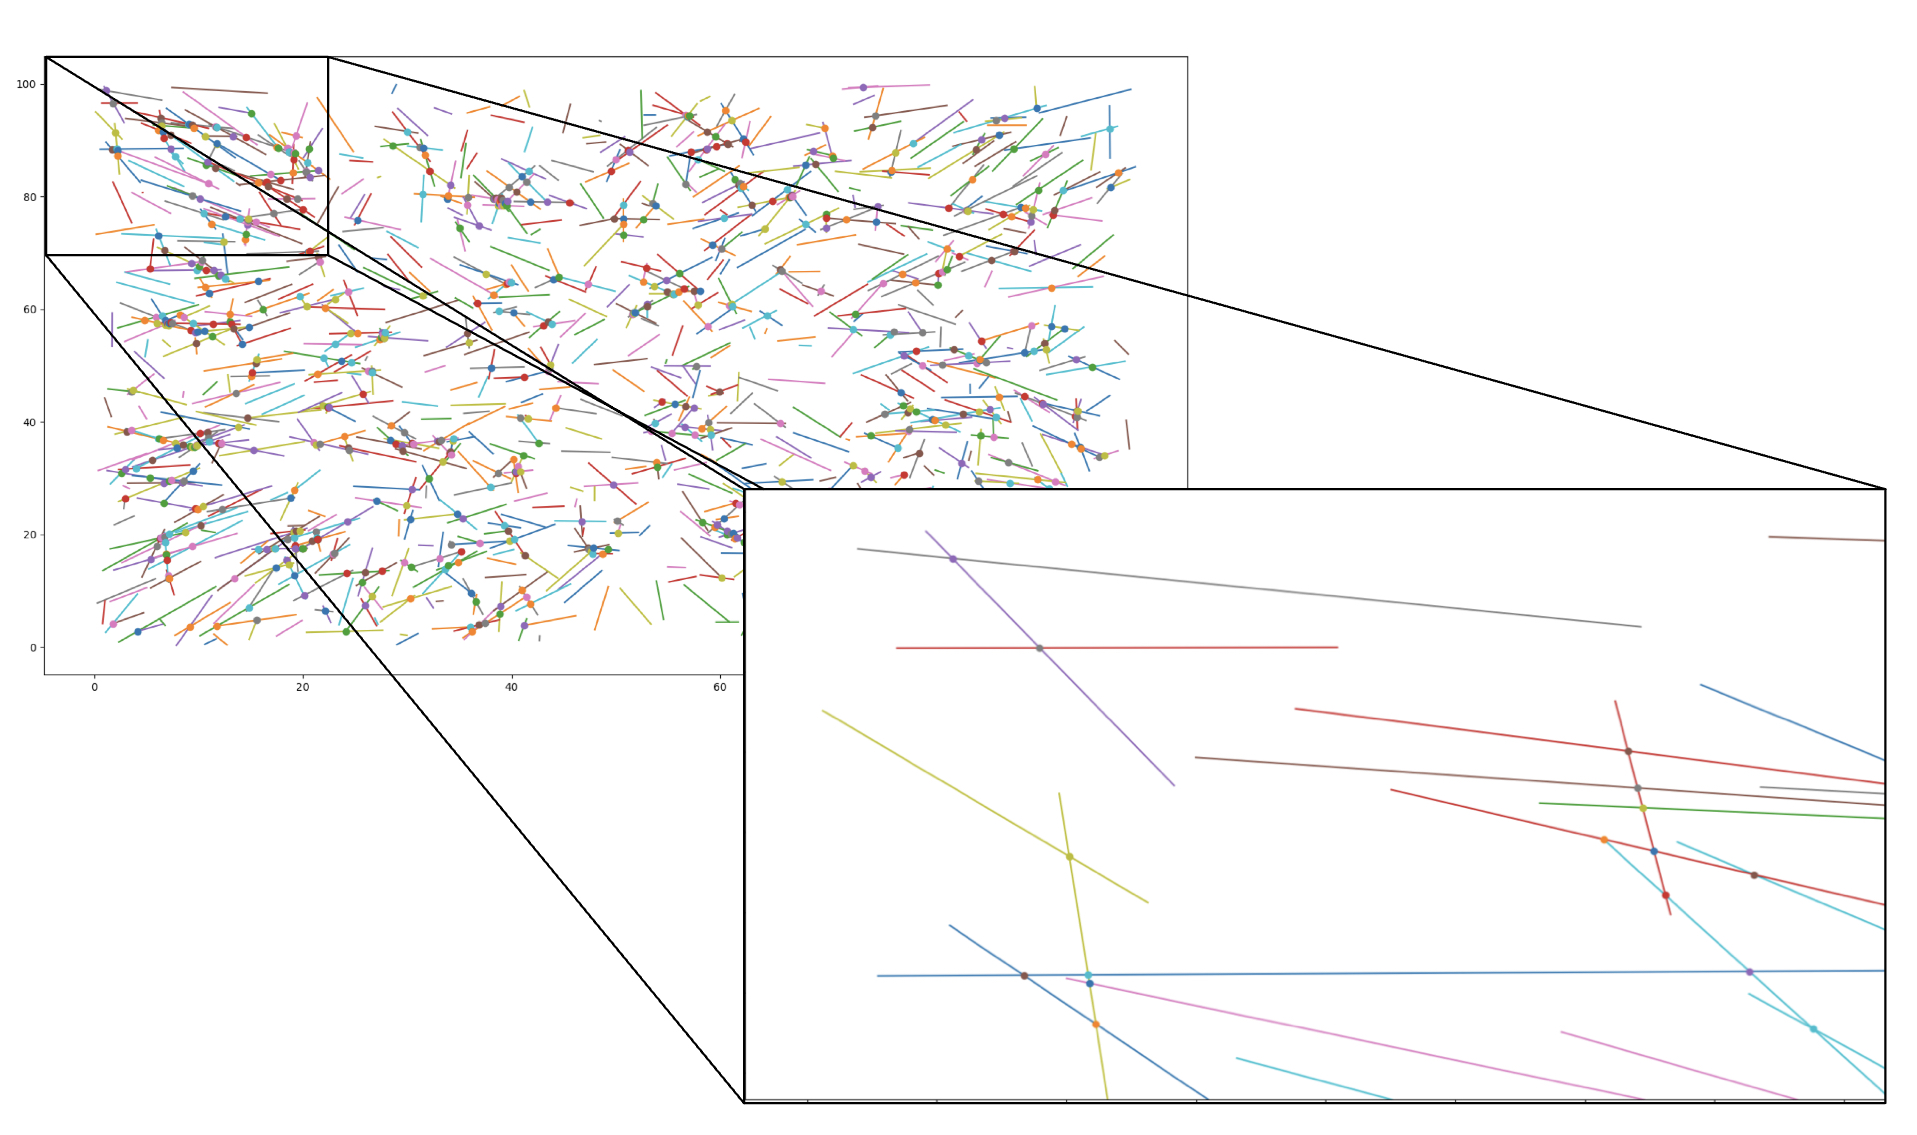
\includegraphics[scale=0.25]{Plot_zoom_and_all.jpeg}
\end{figure}





%\begin{lstlisting}[style=Terminal, caption={testing.cpp: Ausgabe Konsole},captionpos=b, label={lst:ausgabe_test}]
%\end{lstlisting}



\end{document}
